%!TEX root = ./ERL Industrial Robots.tex


%--------------------------------------------------------------------
%--------------------------------------------------------------------
\subsection{Task \emph{Fill a Box with Parts for Manual Assembly (Shared with RoboCup@Work)}}
\label{ssec:TaskFillaBox}

This task reflects one of the primary requisites of a mobile robotic service assistant, i.e., to work together with humans. In this case the goal is to assist humans at a manual assembly workstation.
The robots have to deal with flexible task specifications, especially concerning information about object constellations in source and target locations, and task constraints such as limits on the number of objects allowed to be carried simultaneously, etc. 

%--------------------------------------------------------------------
\subsubsection{Task Description}
\label{sssec:TaskFillaBoxDescription}

The robot has to pick up several parts from different source locations and deliver them to several destination locations. 
%\begin{figure}[!htbp]
%	\begin{center}
%		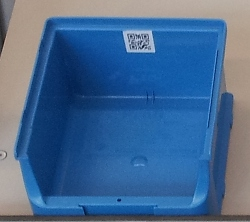
\includegraphics[scale=0.5,angle=0]{fig/Blue_box}
%		\caption{\erlir container with identifier}
%		\label{fig:AidTrayRack2}
%	\end{center}
%\end{figure}

%--------------------------------------------------------------------
\subsubsection{Feature Variation}
\label{sssec:TaskFillaBoxVariation}

%The standardized boxes (see Figure \ref{fig:AidTrayRack2}) can be used for several groups of parts. Because of variations in containing parts (e.g., bearing box variations) the groups of parts in this task vary the same way. 
All objects defined in Section \ref{sssec:PartstoManipulate} will be used in this task.
Several containers (see Section \ref{sssec:EnvironmentObjectstoRecognize}) can be present in the environment and are always associated with a workstation or shelf. It is possible that more than one container is placed on top of a single workstation. Currently, a container itself does to not need to be manipulated or transported by the robot.

For any major competition in which \erlir will be present, additional objects may be used.
Those objects can be found in the rule descriptions of the major competition (e.g. for RoboCup 2016)
%--------------------------------------------------------------------
\subsubsection{Input Provided}
\label{sssec:TaskFillaBoxInput}

The team will be provided with the following information:
%
\begin{itemize}
\item The list of possible parts used in the task;
\item The list of source service areas
\item The list of destination service areas
\end{itemize}

%--------------------------------------------------------------------
\subsubsection{Expected Robot Behavior or Output}
\label{sssec:TaskFillaBoxOutput}

The task execution is triggered by the robot receiving the inventory- and order list from the CFH.
The robot proceeds with collecting the parts from the source locations and transports them to the destination service areas.

%--------------------------------------------------------------------
\subsubsection{Procedures and Rules}
\label{sssec:TaskFillaBoxProcedures}

 There can be multiple obstacles and barrier tapes (color: yellow/black) present in the environment that might block the direct path of the competing robot. The robot must avoid all obstacles or even other robots during the execution of the complete task.
%
\begin{description}
\item[Step 1] The robot will receive an order and inventory from the CFH containing a list of objects to be collected and delivered.
\item[Step 2] The robot must plan the best path to the designated workstation, passing through each storage area where the required objects for a requested product in the list can be found. 
\item[Step 3] The robot must execute the above path, collect the objects and then deliver them to the designated destination locations.
\item[Step 4] The Steps 2 and 3 above must be done for all the objects in the list mentioned above in Step 1.
\end{description}

%--------------------------------------------------------------------
\subsubsection{Communication with CFH}
\label{sssec:CommCFHFillaBox}

For this task benchmark the robot does not have to control any networked device in the environment. Thus, the robot is only supposed to receive the static inventory and order information once. Currently, the robot does not need to update the inventory information.

%--------------------------------------------------------------------
\subsubsection{Acquisition of Benchmarking Data}
\label{sssec:TaskFillaBoxData}
General information on the acquisition of benchmarking data is described in Section \ref{sec:TbmAcquisitionOfData}.

\paragraph{Online Data}
\begin{itemize}
\item No online benchmarking data has to be sent to the CFH during this task benchmark.
\end{itemize}

\paragraph{Offline data} 
The additional information described in the following table has to be logged:
\begin{table}[h]
	\centering
	\begin{footnotesize}
		\begin{tabular}{|l|l|l|l|}
			\hline
			Topic	&	Type		&	Frame Id		&	Notes \\ \hline\hline
			/rockin/notification\tablefootnote{The string with the notification of the perceived object should be in a tab separated string: CLASS OBJECT\_ID X Y THETA} & std\_msgs/String & -- & -- \\ \hline
		\end{tabular}
	\end{footnotesize}
\end{table}

%--------------------------------------------------------------------
\subsubsection{Scoring and Ranking}
\label{sssec:TaskFillaBoxScoring}

Evaluation of the performance of a robot according to this task benchmark is based on performance equivalence classes. Classes are defined in dependence to the number of parts of the product to be assembled actually provided by the robot to the human worker and their order according to the desired one.

%\noindent%
\paragraph{Achievements} The set $A$ of achievements for this task consists of:
%
\begin{itemize}
\item The robot communicates with the CFH throughout the test;
\item The team submits the benchmarking data by the end of the test;
\item The robot picks up a required object from its storage location;
\item The robot places the required objects in its destination area;
\item The robot has correctly collected and delivered all objects
\end{itemize}
%--------------------------------------------------------------------
% EOF
%--------------------------------------------------------------------
